\documentclass[tikz,border=5pt]{standalone}
\usepackage{tikz}
\usetikzlibrary{arrows.meta}

\begin{document}
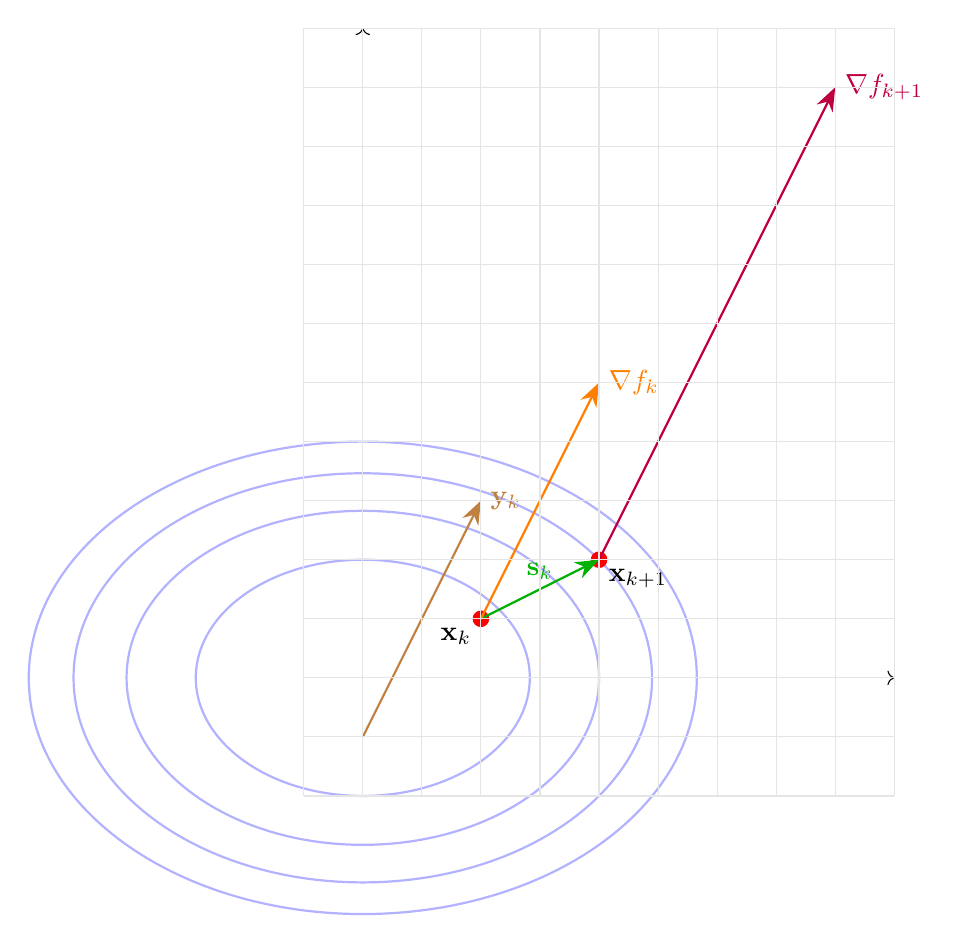
\begin{tikzpicture}[scale=1.5]
    % Define function f(x,y) = 0.5(x^2 + 2y^2)
    % Level curves: x^2 + 2y^2 = 2c
    
    % Draw level curves (ellipses)
    \draw[blue!30, thick] (0,0) ellipse (1.414 and 1); % c = 0.5
    \draw[blue!30, thick] (0,0) ellipse (2 and 1.414); % c = 1
    \draw[blue!30, thick] (0,0) ellipse (2.449 and 1.732); % c = 1.5
    \draw[blue!30, thick] (0,0) ellipse (2.828 and 2); % c = 2
    
    % Define points
    % x_k = (1, 0.5), x_{k+1} = (2, 1)
    \coordinate (xk) at (1, 0.5);
    \coordinate (xk1) at (2, 1);
    
    % Gradients: ∇f(x,y) = (x, 4y)
    % ∇f_k = ∇f(1, 0.5) = (1, 2)
    % ∇f_{k+1} = ∇f(2, 1) = (2, 4)
    \coordinate (gradfk) at (1, 2);
    \coordinate (gradfk1) at (2, 4);
    
    % s_k = x_{k+1} - x_k = (1, 0.5)
    % y_k = ∇f_{k+1} - ∇f_k = (1, 2)
    
    % Draw points
    \fill[red] (xk) circle (2pt);
    \fill[red] (xk1) circle (2pt);
    
    % Labels for points
    \node[below left] at (xk) {$\mathbf{x}_k$};
    \node[below right] at (xk1) {$\mathbf{x}_{k+1}$};
    
    % Draw s_k vector
    \draw[-{Stealth[length=3mm]}, thick, green!70!black] (xk) -- (xk1);
    \node[above, green!70!black] at (1.5, 0.75) {$\mathbf{s}_k$};
    
    % Draw gradient vectors
    \draw[-{Stealth[length=3mm]}, thick, orange] (xk) -- ++(1, 2);
    \node[right, orange] at (2, 2.5) {$\nabla f_k$};
    
    \draw[-{Stealth[length=3mm]}, thick, purple] (xk1) -- ++(2, 4);
    \node[right, purple] at (4, 5) {$\nabla f_{k+1}$};
    
    % Draw y_k vector (∇f_{k+1} - ∇f_k)
    % Start from origin for clarity
    \draw[-{Stealth[length=3mm]}, thick, brown] (0, -0.5) -- ++(1, 2);
    \node[right, brown] at (1, 1.5) {$\mathbf{y}_k$};
    
    % Draw coordinate axes
    \draw[->] (-0.5, 0) -- (4.5, 0);
    \draw[->] (0, -1) -- (0, 5.5);
    
    % Add grid for reference
    \draw[gray!20] (-0.5, -1) grid[step=0.5] (4.5, 5.5);
    
\end{tikzpicture}
\end{document}
